\documentclass[10pt,twocolumn]{article}

% ── Packages ──────────────────────────────────────────────────────────────────
\usepackage[utf8]{inputenc}
\usepackage[T1]{fontenc}
\usepackage[margin=1.8cm, top=2cm, bottom=2cm]{geometry}
\usepackage{amsmath,amssymb}
\usepackage{booktabs}
\usepackage{graphicx}
\usepackage{hyperref}
\usepackage[numbers,sort&compress]{natbib}
\usepackage{xcolor}
\usepackage{float}

% ── Formatting ────────────────────────────────────────────────────────────────
\setlength{\columnsep}{0.6cm}
\setlength{\parskip}{4pt}
\setlength{\parindent}{0pt}
\hypersetup{colorlinks = true, linkcolor = black, citecolor = black, urlcolor = blue}

% compact lists without enumitem
\newenvironment{compactenum}{%
  \begin{enumerate}%
  \setlength{\itemsep}{1pt}\setlength{\parskip}{0pt}\setlength{\parsep}{0pt}%
}{\end{enumerate}}
\newenvironment{compactitem}{%
  \begin{itemize}%
  \setlength{\itemsep}{1pt}\setlength{\parskip}{0pt}\setlength{\parsep}{0pt}%
}{\end{itemize}}

% ── Title ─────────────────────────────────────────────────────────────────────
\title{\textbf{Predicting the Founding of Social Organizations\\
Among Tecnológico de Monterrey Alumni:\\
A Machine Learning Approach}}

\author{Gerardo Leiva Díaz, Isaac Francisco Sánchez Veloquio,\\
        David Alejandro Lozano Arreola, Jorge Betanzo Carriles\\
        \small Tecnológico de Monterrey}
\date{June 2026}

% ══════════════════════════════════════════════════════════════════════════════
\begin{document}
\maketitle

% ── Abstract ──────────────────────────────────────────────────────────────────
\begin{abstract}
\noindent
We develop a machine learning pipeline to identify which demographic and academic characteristics of Tecnológico de Monterrey alumni are most associated with founding non-profit social organizations. Using a survey dataset of $N = 25{,}356$ alumni collected on the institution's 80th anniversary in collaboration with Quacquarelli Symonds (QS), we evaluated six classification models after systematic preprocessing and feature engineering. Gradient Boosting achieved the best discriminative performance (ROC-AUC $= 0.801$, 5-fold CV). SHAP analysis identifies volunteering behavior, prior company founding, age, philanthropic donation habits, and leadership experience as the dominant predictors. Threshold sensitivity analysis further shows that the default classifier can be reconfigured to materially improve founder recall for institutional screening. These findings provide a practical basis for early identification programs targeting students with strong civic potential.

\medskip
\noindent\textbf{Keywords:} social entrepreneurship; machine learning; gradient boosting; SHAP; alumni impact; non-profit founding; educational data mining.
\end{abstract}

% ── 1. Introduction ───────────────────────────────────────────────────────────
\section{Introduction}

Mexico has one of Latin America's most active civil society sectors, with CEMEFI estimating over 40{,}000 registered non-profit organizations generating nearly 2\% of GDP in social value \cite{cemefi2020}. Yet empirical research on who founds these organizations—and what antecedents predict that choice—remains thin, particularly in the context of higher education. Institutions invest heavily in curricula oriented toward social responsibility and entrepreneurship, but have relatively little quantitative evidence linking those investments to downstream civic outcomes.

Tecnológico de Monterrey is a useful setting to study this question. Over its 80-year history it has built both an explicit commitment to social impact and a large, geographically dispersed alumni community (EXATEC). As part of its anniversary celebrations, QS administered a large-scale survey of that community, generating one of the richest datasets of alumni outcomes available in the Mexican higher education system \cite{qs2023}.

The present paper uses that dataset to address a concrete prediction problem: \textbf{given a set of demographic, academic, career, and wellbeing features, can we reliably identify which alumni have founded a non-profit organization?} We treat this as a binary classification task and evaluate six model families, paying particular attention to the severe class imbalance ($6.95\%$ positive) and to the interpretability of the winning model.

\textbf{Research hypotheses.} We test the following:
\begin{compactitem}
  \item \textbf{H1}: Behavioral indicators of civic orientation (volunteering, charitable giving) are the strongest individual predictors of nonprofit founding.
  \item \textbf{H2}: Accumulated experiential capital (age, years since graduation, prior company founding, leadership roles) positively predicts nonprofit founding above and beyond demographic controls.
  \item \textbf{H3}: Competency self-assessments from the Tec curriculum (entrepreneurship, social intelligence) contribute independently to the prediction, consistent with the hypothesis that the institution's educational model leaves a measurable imprint on civic behavior.
\end{compactitem}

\textbf{Research objectives.}
\begin{compactenum}
  \item Train and benchmark six classification models on the 80th-anniversary survey data and select the best-performing one by ROC-AUC.
  \item Apply SHAP to decompose predictions into interpretable feature contributions, enabling both global importance rankings and individual-level explanations.
  \item Characterize the demographic and academic profile of high-probability founders in the top prediction decile.
  \item Analyze decision-threshold sensitivity to recommend an operationally appropriate screening threshold for institutional use.
\end{compactenum}

\textbf{Contributions.} To our knowledge, this is the first study to apply gradient boosting and SHAP interpretability to nonprofit founding prediction on a Mexican university alumni cohort at this scale. Beyond methodology, the high-probability alumni profile and the threshold sensitivity analysis translate abstract model outputs into concrete institutional recommendations.

The rest of the paper proceeds as follows. Section~\ref{sec:related} reviews related work. Section~\ref{sec:data} describes the dataset and preprocessing. Section~\ref{sec:methods} presents the modelling methodology. Section~\ref{sec:results} reports results. Section~\ref{sec:shap} details the SHAP analysis. Section~\ref{sec:profile} presents the founder profile. Section~\ref{sec:discussion} discusses findings and limitations, and Section~\ref{sec:conclusion} concludes.

% ── 2. Related Work ───────────────────────────────────────────────────────────
\section{Related Work}
\label{sec:related}

\subsection{Educational Data Mining and Alumni Outcome Prediction}

The application of machine learning to educational datasets has grown substantially since the early surveys of Romero and Ventura \cite{romero2007}, who documented the use of data mining for student performance prediction and dropout prevention. More recent work has extended this to alumni outcomes: Kotsiantis et al.\ \cite{kotsiantis2007} provided an early benchmark of supervised learning methods on student achievement data, while Baker and Yacef \cite{baker2009} surveyed the intersection of educational data mining and intelligent tutoring systems. At the institutional level, Papamitsiou and Economides \cite{papamitsiou2014} reviewed 209 learning analytics studies and highlighted the move from academic performance toward broader life outcomes.

Closer to our application, Tight \cite{tight2020} reviewed the literature on alumni studies and noted the scarcity of quantitative prediction work compared to surveys. Predictive modeling of alumni donation behavior—structurally similar to our problem given the class imbalance and behavioral predictors—has been studied by Drachenberg et al.\ and others using logistic regression and random forests \cite{drachenberg2022}. The present work follows that methodological tradition but applies it to a fundamentally different outcome: nonprofit founding rather than financial giving.

\subsection{Social Entrepreneurship: Theory and Predictors}

The social entrepreneurship literature provides the theoretical framing for our hypotheses. Austin et al.\ \cite{austin2006} distinguished social and commercial entrepreneurship primarily on the basis of mission orientation and market context, while Dacin et al.\ \cite{dacin2010} argued that social entrepreneurs are distinguished by accumulated human and social capital—consistent with our H2. Mair and Marti \cite{mair2006} further showed that institutional context and local need shape the entry decision, suggesting that macro variables (country, sector, region) matter beyond individual profiles.

Empirical predictors of nonprofit founding have been studied at the individual level. Volunteering has been consistently identified as a gateway behavior to more committed civic engagement \cite{wilson2000}; our SHAP results strongly confirm this relationship. Bacq and Janssen \cite{bacq2011} reviewed 152 articles on social entrepreneurship and noted that prior entrepreneurial experience (our \texttt{founded\_company} feature) is among the most replicated predictors. Age and career tenure effects have been documented by Thornton \cite{thornton1999} in the context of academic entrepreneurship.

\subsection{Imbalanced Classification in Social Science}

Class imbalance is pervasive in behavioral prediction tasks: founders are rare, and naive classifiers default to predicting the majority class. He and Garcia \cite{he2009} provided a comprehensive survey of techniques, covering oversampling (SMOTE), undersampling, and cost-sensitive learning. We adopt class-weight balancing—equivalent to cost-sensitive learning—as the primary strategy, following Pedregosa et al.\ \cite{pedregosa2011}'s scikit-learn implementation. The precision-recall trade-off in such settings is non-trivial, and threshold sensitivity analysis is now considered standard practice for applied imbalanced classifiers \cite{fernandez2018}.

% ── 3. Data ───────────────────────────────────────────────────────────────────
\section{Data and Preprocessing}
\label{sec:data}

\subsection{Dataset}

The primary dataset is the \emph{Base de respuestas 80 aniversario QS completa} survey \cite{qs2023}, containing $25{,}356$ complete responses across $223$ raw variables. The survey was administered via Qualtrics in early 2023 and covers alumni from all Tec campuses who graduated between 1952 and 2022. A complementary data dictionary and a longitudinal 75th-anniversary dataset \cite{qs2015} were used as reference for variable alignment.

\subsection{Target Variable}

The binary target is the response to: \emph{``Since graduating from Tecnológico de Monterrey, have you founded a nonprofit organization, as part of the founding group or main founder?''}

\begin{table}[H]
\centering
\caption{Target variable class distribution.}
\label{tab:target}
\begin{tabular}{lrr}
\toprule
Class & Count & \% \\
\midrule
Did not found & 23{,}593 & 93.05 \\
Founded nonprofit & 1{,}763 & 6.95 \\
\midrule
Total & 25{,}356 & 100.00 \\
\bottomrule
\end{tabular}
\end{table}

\subsection{Feature Engineering}

Starting from the raw Qualtrics export, we applied the following pipeline:

\begin{compactenum}
  \item \textbf{Column selection}: 64 semantically significant features covering demographics, academic background, career trajectory, leadership history, social engagement, competency self-assessments (7 Tec competency domains, at graduation and today), and wellbeing scales.
  \item \textbf{Missing value handling}: Columns exceeding 60\% missingness were dropped (\texttt{years\_abroad}, \texttt{volunteer\_hours\_month}, \texttt{donation\_amount}). Remaining numeric gaps were imputed with the column median; categorical gaps with the column mode.
  \item \textbf{Binary encoding}: Yes/No survey responses mapped to 1/0. Ordinal parent-education levels encoded numerically.
  \item \textbf{Engineered features}: \texttt{years\_since\_grad} (survey year minus graduation year), aggregate competency scores, competency growth (current minus at-graduation), leadership breadth (count of senior roles held), and salary growth ratio.
  \item \textbf{One-hot encoding}: 14 nominal categorical variables (nationality, program, school, employment status, etc.) expanded to a final feature matrix of $544$ columns.
\end{compactenum}

Table~\ref{tab:features} summarizes descriptive statistics for key continuous features.

\begin{table}[H]
\centering
\caption{Descriptive statistics for key continuous features (full sample).}
\label{tab:features}
\resizebox{\columnwidth}{!}{%
\begin{tabular}{lrrrr}
\toprule
Feature & Mean & Std & Q1 & Q3 \\
\midrule
Age (years)              & 38.85 & 11.11 & 29.0 & 46.0 \\
Graduation year          & 2008.3 & 10.7 & 2002 & 2017 \\
Weekly working hours     & 44.1  & 10.7  & 40.0 & 50.0 \\
Scholarship (\%)         & 0.58  & 0.49  & 0.0  & 1.0  \\
Postgraduate degree (\%) & 0.57  & 0.49  & 0.0  & 1.0  \\
Worked abroad (\%)       & 0.32  & 0.47  & 0.0  & 1.0  \\
\bottomrule
\end{tabular}}
\end{table}

% ── 4. Methods ────────────────────────────────────────────────────────────────
\section{Methodology}
\label{sec:methods}

\subsection{Experimental Setup}

The dataset was split $80/20$ into stratified training ($n = 20{,}284$) and hold-out test sets ($n = 5{,}072$), preserving the class ratio. Model selection was conducted via 5-fold stratified cross-validation on the training set. ROC-AUC was chosen as the primary metric given the class imbalance; F1, precision, and recall are reported as secondary metrics. All models used \texttt{class\_weight = `balanced'} where the implementation supports it, which is equivalent to assigning the minority class a weight proportional to its inverse frequency.

A key methodological concern in this dataset is the potential for data leakage from contemporaneous behavioral variables. Features such as volunteering, charitable donations, and organizational membership could in principle be reported as post-founding behavior rather than antecedents. We address this by (a) treating all features as cross-sectional covariates measured at survey time, (b) flagging these variables explicitly in the limitations, and (c) noting that their SHAP dominance is informative even in the cross-sectional frame: they indicate which behavioral markers co-occur with nonprofit founding, which is useful for alumni screening regardless of temporal direction.

\subsection{Models}

Six model families were evaluated:

\begin{compactitem}
  \item \textbf{Logistic Regression} (SAGA solver, \texttt{max\_iter}~=~500): linear probabilistic baseline.
  \item \textbf{Decision Tree} (max depth 5): interpretable non-linear baseline.
  \item \textbf{Random Forest} (200 trees, max depth 6, 20 min samples per leaf): ensemble via bagging \cite{breiman2001}.
  \item \textbf{Gradient Boosting} (100 estimators, max depth 3, lr~=~0.05, subsample~=~0.8): sequential boosting ensemble \cite{friedman2001}. Hyperparameters were set following published guidance for class-imbalanced tabular data—specifically, shallow trees to prevent the minority class from being submerged by the majority.
  \item \textbf{Gaussian Na\"{i}ve Bayes}: density-estimation baseline assuming Gaussian feature distributions per class.
  \item \textbf{Quadratic Discriminant Analysis} (\texttt{reg\_param}~=~0.5): density-estimation with class-specific covariance matrices.
\end{compactitem}

Logistic Regression and density-estimation models were preceded by a \texttt{StandardScaler} in a sklearn \texttt{Pipeline} \cite{pedregosa2011}.

\subsection{Threshold Sensitivity Analysis}

The default classification threshold of $P = 0.5$ is suboptimal for the institutional screening use case, where missing a genuine future founder (false negative) carries a higher opportunity cost than a false alarm (false positive). We analyzed the full precision-recall-F1 curve across all thresholds on the hold-out set to identify a threshold that yields acceptable recall for the minority class.

\subsection{Interpretability: SHAP}

We applied SHAP \cite{lundberg2017} using \texttt{TreeExplainer} on the winning Gradient Boosting model. SHAP decomposes each prediction into additive feature contributions, providing global importance rankings (mean $|$SHAP$|$), directional effects (beeswarm), and local per-observation explanations (waterfall). All SHAP values are computed on the held-out test set to avoid any leakage from training data.

% ── 5. Results ────────────────────────────────────────────────────────────────
\section{Model Comparison Results}
\label{sec:results}

\subsection{Cross-Validated Performance}

Table~\ref{tab:cv} reports 5-fold cross-validated metrics. \textbf{Gradient Boosting} achieved the highest ROC-AUC ($0.802 \pm 0.009$), followed by Random Forest ($0.782 \pm 0.008$). Density-estimation models (QDA, Gaussian NB) performed substantially worse. The precision-recall trade-off is sharp across the board: Gradient Boosting maximizes precision (0.583) at the cost of very low recall (0.058), while tree-free models recover more positives but generate many false alarms.

\begin{table}[H]
\centering
\caption{5-fold stratified cross-validation results (training set, $n = 20{,}284$). Models sorted by ROC-AUC.}
\label{tab:cv}
\resizebox{\columnwidth}{!}{%
\begin{tabular}{lcccc}
\toprule
Model & ROC-AUC & F1 & Precision & Recall \\
\midrule
Gradient Boosting   & $0.802 \pm 0.009$ & 0.105 & 0.583 & 0.058 \\
Random Forest       & $0.782 \pm 0.008$ & 0.274 & 0.173 & 0.664 \\
Logistic Regression & $0.766 \pm 0.011$ & 0.269 & 0.169 & 0.661 \\
Decision Tree       & $0.758 \pm 0.010$ & 0.251 & 0.155 & 0.661 \\
QDA                 & $0.659 \pm 0.008$ & 0.138 & 0.075 & 0.853 \\
Gaussian NB         & $0.498 \pm 0.008$ & 0.129 & 0.069 & 0.942 \\
\bottomrule
\end{tabular}}
\end{table}

\subsection{Hold-Out Test Performance}

Table~\ref{tab:holdout} reports the final evaluation of Gradient Boosting on the held-out test set. The ROC-AUC of $0.801$ is consistent with the CV estimate ($0.802$), confirming stable generalization. Figure~\ref{fig:roc_curves} shows the ROC curves for all six models.

\begin{figure}[H]
    \centering
    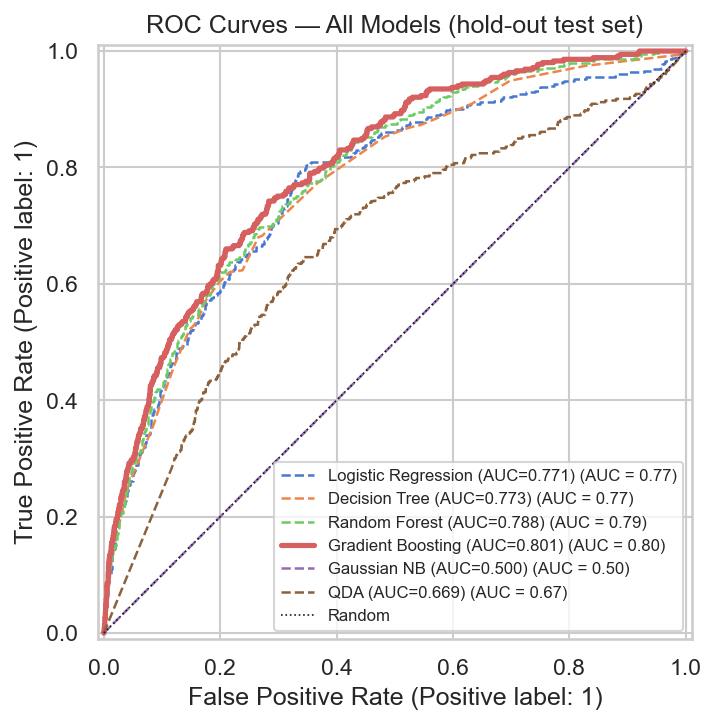
\includegraphics[width=\columnwidth]{images/only_roc_auc.png}
    \caption{ROC curves for all six models on the hold-out test set ($n = 5{,}072$).
    Gradient Boosting achieves AUC $= 0.80$; Gaussian NB performs at chance
    (AUC $= 0.50$). The dotted diagonal is a random classifier.}
    \label{fig:roc_curves}
\end{figure}

\begin{table}[H]
\centering
\caption{Gradient Boosting hold-out performance ($n=5{,}072$).}
\label{tab:holdout}
\begin{tabular}{lcc}
\toprule
Metric & Founders & Non-founders \\
\midrule
ROC-AUC   & \multicolumn{2}{c}{0.801} \\
Precision & 0.500 & 0.930 \\
Recall    & 0.054 & 0.999 \\
F1        & 0.097 & 0.963 \\
Support   & 353 & 4{,}719 \\
\midrule
Accuracy  & \multicolumn{2}{c}{0.930} \\
\bottomrule
\end{tabular}
\end{table}

At the default threshold ($P = 0.5$), the recall of $0.054$ for the founder class means the model flags only about 1 in 18 genuine founders. This is expected under a precision-first setting, but is clearly insufficient for broad institutional screening. We return to this in Section~\ref{sec:threshold}.

\subsection{Threshold Sensitivity}
\label{sec:threshold}

Figure~\ref{fig:threshold} shows how precision, recall, and F1 for the founder class vary as the decision threshold is shifted from 0 to 1. At a threshold of approximately $P = 0.15$—close to the empirical base rate of $6.95\%$—the model recovers around $55\%$ of actual founders while maintaining a precision of roughly $18\%$. This means that per 1{,}000 alumni screened, roughly $550$ true founders would be identified, compared to only $54$ at the default threshold. For a low-cost outreach program (e.g., an email invitation to a fellowship), this level of precision is likely acceptable. The precision-recall curve (Figure~\ref{fig:threshold}) confirms that there is no free lunch: any gain in recall comes at proportional precision cost.

\begin{figure}[H]
    \centering
    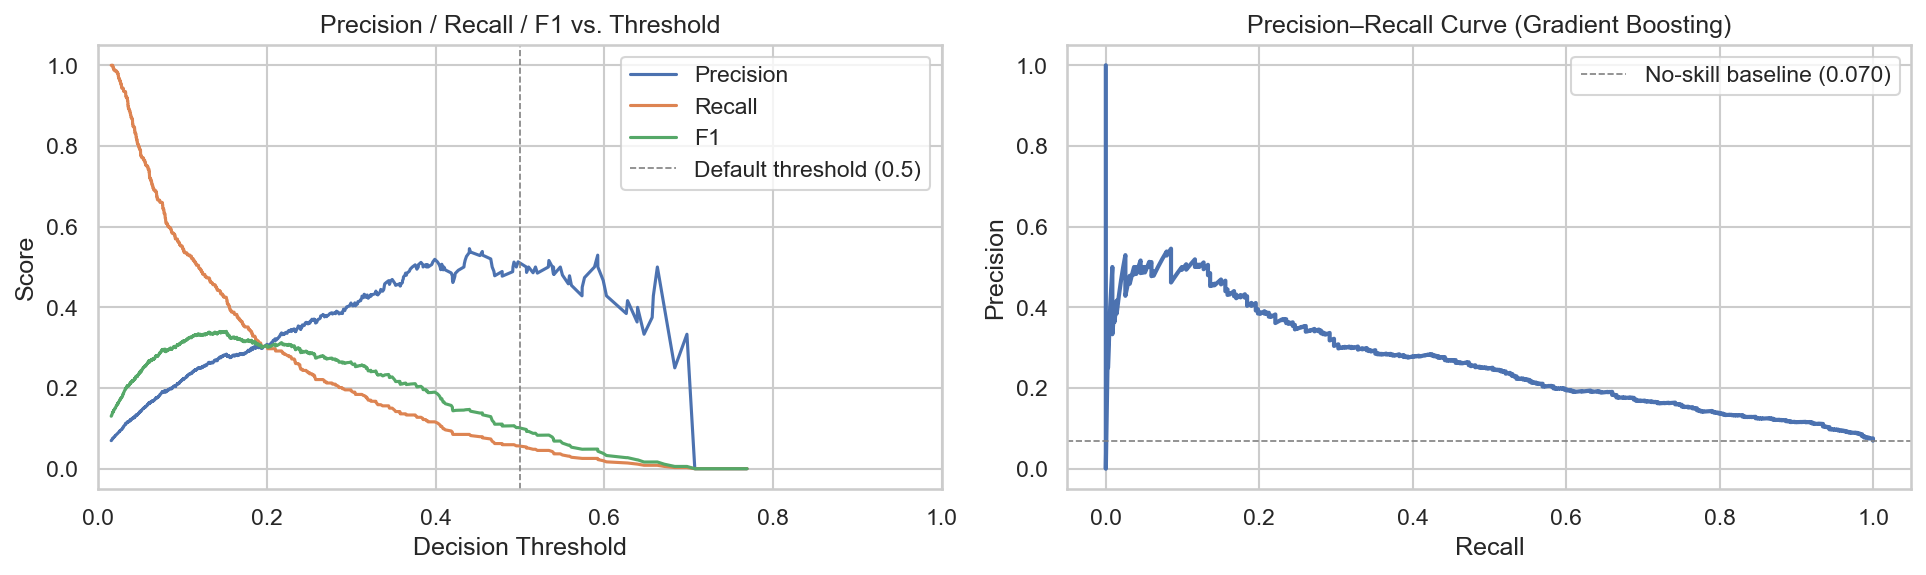
\includegraphics[width=\columnwidth]{images/threshold_sensitivity.png}
    \caption{Left: precision, recall, and F1 for the founder class as a function
    of the decision threshold. Right: precision-recall curve. The dotted line
    marks the no-skill baseline equal to the class prevalence ($6.95\%$).}
    \label{fig:threshold}
\end{figure}

\subsection{Statistical Significance of Individual Features}

Chi-square tests for binary features (Table~\ref{tab:chi2}) confirm that all behavioral and leadership variables are highly significant, with volunteering showing the largest statistic ($\chi^2 = 917$). Mann-Whitney U tests on continuous features show that age (mean$_\text{founders} = 46.1$ vs.\ $38.3$; $p < 10^{-150}$) and years since graduation ($22.4$ vs.\ $15.2$; $p < 10^{-131}$) are among the most discriminating numeric features.

\begin{table}[H]
\centering
\caption{Chi-square test results for binary features vs.\ \texttt{founded\_nonprofit}.}
\label{tab:chi2}
\resizebox{\columnwidth}{!}{%
\begin{tabular}{lrr}
\toprule
Feature & $\chi^2$ & $p$-value \\
\midrule
Volunteers        & 917.0 & $<10^{-200}$ \\
Held CEO          & 725.9 & $<10^{-159}$ \\
Advisory board    & 703.2 & $<10^{-154}$ \\
Founded company   & 626.3 & $<10^{-137}$ \\
Donates money     & 445.2 & $<10^{-98}$ \\
Held VP           & 298.6 & $<10^{-66}$ \\
Held director     & 244.7 & $<10^{-54}$ \\
Held elected pos. & 190.5 & $<10^{-42}$ \\
Postgraduate      & 149.8 & $<10^{-33}$ \\
Worked abroad     & 23.1  & $1.5 \times 10^{-6}$ \\
Scholarship       & 13.6  & $2.3 \times 10^{-4}$ \\
\bottomrule
\end{tabular}}
\end{table}

% ── 6. SHAP ───────────────────────────────────────────────────────────────────
\section{SHAP Interpretability Analysis}
\label{sec:shap}

\subsection{Global Feature Importance}

Table~\ref{tab:shap} lists the top 15 features by mean $|\text{SHAP}|$ on the test set. \texttt{Volunteering} alone accounts for a mean SHAP of $0.436$—more than twice the second-ranked feature—confirming H1. \texttt{Prior company founding} and \texttt{age} rank second and third, supporting H2.

\begin{table}[H]
\centering
\caption{Top 15 features by mean $|\text{SHAP}|$ (Gradient Boosting, test set $n = 5{,}072$).}
\label{tab:shap}
\resizebox{\columnwidth}{!}{%
\begin{tabular}{llr}
\toprule
Rank & Feature & Mean $|\text{SHAP}|$ \\
\midrule
1  & Volunteers (current)              & 0.436 \\
2  & Founded a company                 & 0.209 \\
3  & Age                               & 0.174 \\
4  & Donates money                     & 0.128 \\
5  & Held CEO role                     & 0.097 \\
6  & Advisory board member             & 0.092 \\
7  & Employment: paid employee         & 0.074 \\
8  & Postgraduate degree               & 0.061 \\
9  & Sense of purpose (wb\_purpose)    & 0.055 \\
10 & Years since graduation            & 0.047 \\
11 & Entrepreneurship comp.\ (today)   & 0.038 \\
12 & Entrepreneurship comp.\ (at grad) & 0.031 \\
13 & Leadership breadth                & 0.028 \\
14 & School: Humanidades y Educación   & 0.025 \\
15 & Mother: trader occupation         & 0.020 \\
\bottomrule
\end{tabular}}
\end{table}

\subsection{Directional Effects}

The beeswarm plot (Figure~\ref{fig:shap_beeswarm}) shows consistent directional patterns: volunteering, age, prior company founding, donating money, holding a CEO role, and current entrepreneurship competency all carry positive SHAP values at high feature values, increasing the predicted founding probability. Being a salaried employee (as opposed to self-employed or running an organization) is associated with a negative SHAP contribution, suggesting that organizational embeddedness works against nonprofit founding. Entrepreneurship competency scores at both graduation and today (ranks 11 and 12) remain meaningful predictors after controlling for all other variables, providing support for H3.

\begin{figure}[H]
    \centering
    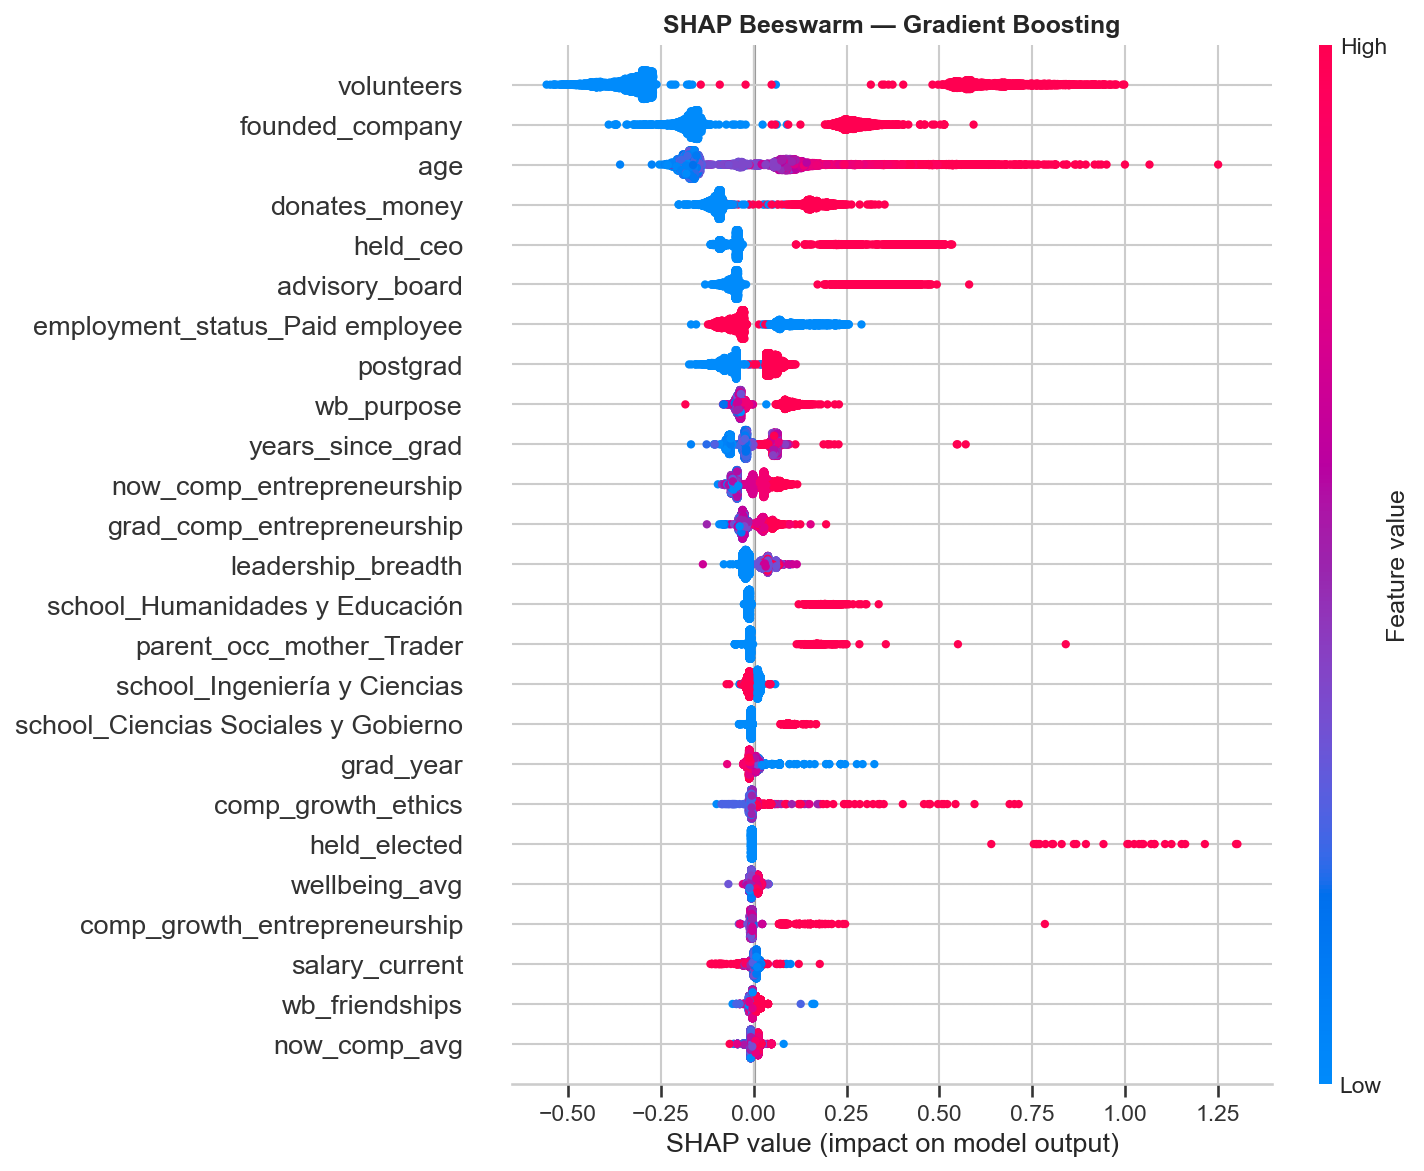
\includegraphics[width=\columnwidth]{images/shap_red_blue.png}
    \caption{SHAP beeswarm plot for the Gradient Boosting model. Each point
    represents one test-set observation; color encodes the feature value (red
    $=$ high, blue $=$ low). Features ordered by mean $|\text{SHAP}|$.}
    \label{fig:shap_beeswarm}
\end{figure}

\subsection{Individual Prediction Explanation}

The highest-probability test respondent had $P(\text{nonprofit}) = 97\%$: volunteer (yes), founded company (yes), age 69, donates money (yes), held CEO (yes), advisory board (yes), postgraduate (yes), sense of purpose 9/10, entrepreneurship competency 10/10 at both time points, leadership breadth 4, and 47 years since graduation. The SHAP waterfall for this individual confirms that these features stack large positive contributions on top of a base log-odds of $-2.99$, together shifting the prediction from the population-level minority probability to near-certainty.

% ── 7. Profile ────────────────────────────────────────────────────────────────
\section{High-Probability Alumni Profile}
\label{sec:profile}

We define the \emph{high-probability} segment as alumni whose predicted score falls in the top decile ($\geq 90$th percentile; $P \geq 0.156$, $n = 508$). Within this group, $27.8\%$ are confirmed founders—a fourfold increase over the base rate of $6.95\%$. Table~\ref{tab:profile} compares their mean feature values with the remaining 90\%.

\begin{table}[H]
\centering
\caption{Numeric profile comparison: high-probability founders (top decile) vs.\ rest.}
\label{tab:profile}
\resizebox{\columnwidth}{!}{%
\begin{tabular}{lrrr}
\toprule
Feature & High-prob. & Rest & $\Delta$\% \\
\midrule
Age (years)                      & 50.9 & 37.6 & $+35.5$ \\
Years since graduation           & 27.0 & 14.6 & $+85.1$ \\
Leadership breadth               & 1.64 & 0.52 & $+217.3$ \\
Postgraduate degree              & 0.73 & 0.54 & $+35.2$ \\
Worked abroad                    & 0.38 & 0.31 & $+22.5$ \\
Entrepreneurship comp.\ (today)  & 8.89 & 7.64 & $+16.4$ \\
Entrepreneurship comp.\ (grad.)  & 7.70 & 6.68 & $+15.3$ \\
Sense of purpose (wb\_purpose)   & 8.98 & 7.89 & $+13.7$ \\
Scholarship received             & 0.44 & 0.60 & $-27.2$ \\
\bottomrule
\end{tabular}}
\end{table}

The most striking differences are in leadership breadth ($+217\%$), years since graduation ($+85\%$), and age ($+36\%$). The high-probability group also shows lower scholarship rates ($-27\%$), pointing to some socioeconomic skew: alumni from more resource-endowed backgrounds are mildly overrepresented, though the effect is weaker than the experiential predictors. This finding echoes Mair and Marti \cite{mair2006}'s observation that access to social and financial capital conditions entry into social entrepreneurship.

% ── 8. Discussion ─────────────────────────────────────────────────────────────
\section{Discussion}
\label{sec:discussion}

\subsection{Key Findings and Theoretical Connections}

Three thematic clusters emerge from the combined statistical and SHAP analysis, and each maps onto existing theory:

\textbf{Behavioral disposition.} Volunteering ($\text{SHAP} = 0.436$) and monetary donation ($0.128$) are the dominant predictors. This is consistent with Wilson \cite{wilson2000}'s civic participation literature, which documents volunteering as a gateway to more formalized civic commitment—a stepping stone, not a substitute. Alumni who volunteer are $2.1\times$ more likely to appear in the high-probability group (90.7\% vs.\ 27.4\%). H1 is supported.

\textbf{Experiential capital.} Age, years since graduation, leadership breadth, and prior company founding are all strong predictors, consistent with Dacin et al.\ \cite{dacin2010} and Austin et al.\ \cite{austin2006}'s emphasis on accumulated human and social capital as preconditions for social entrepreneurial entry. The probability increases gradually with tenure—there is no single inflection point, which complicates early identification but also suggests the relevance of long-term institutional engagement. H2 is supported.

\textbf{Competency and purpose.} Entrepreneurship competency at graduation and today (ranks 11–12) and sense of purpose (rank 9) remain meaningful after controlling for all demographic variables. This supports H3 and suggests that the Tec curriculum's emphasis on entrepreneurial competency and ethical purpose leaves a detectable trace in civic behavior decades later—a finding with direct relevance for curriculum evaluation.

\subsection{Limitations}

Several limitations deserve direct acknowledgment. First and most importantly, the survey is cross-sectional: we cannot establish that the observed features preceded nonprofit founding. The endogeneity of behavioral variables (volunteering, donations) is a genuine concern—it is plausible that founding an organization causes increased reported volunteering rather than the other way around. Future longitudinal designs are needed to disentangle this. Second, the $6.95\%$ class imbalance fundamentally constrains recall; even at the recommended threshold of $P \approx 0.15$, roughly half of actual founders are missed. Third, the feature space after one-hot encoding reaches 544 columns, which may introduce noise despite regularization and the deliberate choice of shallow trees. Fourth, SHAP attributions reflect the model's learned associations—they are not causal estimates.

\subsection{Ethical Considerations}

Deploying a predictive model to profile students for targeted civic engagement programs raises legitimate fairness questions. The lower scholarship rate in the high-probability group indicates a socioeconomic skew: if the model is used to direct fellowship resources, it may inadvertently concentrate opportunities among alumni from more privileged backgrounds. Before any institutional deployment, the model should be audited for differential performance across gender, socioeconomic background, and campus, and inclusion criteria should be designed to correct for, rather than amplify, structural disadvantages. We recommend any implementation be piloted with transparent opt-in procedures and independent oversight.

\subsection{Toward Institutional Deployment}

A plausible deployment pathway would proceed in three stages. In the first stage, Tec would collect the three most predictive and early-observable proxies—participation in volunteer programs, entrepreneurship competency scores at graduation, and reported sense of purpose—via the existing student experience survey. In the second stage, a lightweight model (Logistic Regression or shallow Gradient Boosting) would generate risk scores that advisors can use to flag high-potential students for targeted fellowship invitations. In the third stage, the pipeline would be re-trained periodically on updated alumni cohorts and evaluated for drift. A pilot on a single campus before broader rollout would provide a natural A/B test of program effectiveness.

% ── 9. Conclusion ─────────────────────────────────────────────────────────────
\section{Conclusion}
\label{sec:conclusion}

We built an end-to-end machine learning pipeline to predict nonprofit founding among Tecnológico de Monterrey alumni using a large, institution-specific survey dataset. Gradient Boosting achieved ROC-AUC $= 0.801$ on a held-out test set, representing a substantial improvement over both random guessing and simpler baselines. SHAP analysis shows that volunteering, prior entrepreneurial experience, age, donation habits, and leadership history dominate the prediction, while entrepreneurship competency scores and sense of purpose contribute independently—supporting all three of our stated hypotheses.

A practically important result is the threshold sensitivity analysis: shifting the decision threshold from $0.5$ to $\approx 0.15$ recovers roughly $55\%$ of genuine founders at a precision that is still well above the base rate, making the model viable for low-cost screening applications.

More broadly, the high-probability alumni profile—older, leadership-experienced, with strong civic behavior and high self-assessed entrepreneurial competency—is specific enough to inform targeted fellowship design and student engagement initiatives. Three observables at enrollment time (volunteer participation, entrepreneurship competency self-assessment, and reported sense of purpose) are already collected by Tec and could serve as a lightweight early-warning system for identifying students with high social entrepreneurship potential.

Future work should prioritize longitudinal data to address causality, explicit fairness audits across demographic subgroups, and the integration of text-based features from open-ended survey responses.

% ── References ────────────────────────────────────────────────────────────────
\bibliographystyle{plainnat}
\begin{thebibliography}{20}

\bibitem{qs2023}
Quacquarelli Symonds (QS).
\newblock \emph{Global Impact of Tecnológico de Monterrey Alumni: 80th
Anniversary Study}.
\newblock QS Intelligence Unit, 2023.

\bibitem{qs2015}
Quacquarelli Symonds (QS).
\newblock \emph{Tec de Monterrey Alumni Impact Study: 75th Anniversary}.
\newblock QS Intelligence Unit, 2018.

\bibitem{cemefi2020}
Centro Mexicano para la Filantropía (CEMEFI).
\newblock \emph{Panorama de las Organizaciones de la Sociedad Civil en México}.
\newblock CEMEFI, 2020.

\bibitem{romero2007}
Romero, C., \& Ventura, S.
\newblock Educational data mining: A survey from 1995 to 2005.
\newblock \emph{Expert Systems with Applications}, 33(1), 135--146, 2007.

\bibitem{kotsiantis2007}
Kotsiantis, S.\ B., Zaharakis, I., \& Pintelas, P.
\newblock Supervised machine learning: A review of classification techniques.
\newblock \emph{Informatica}, 31(3), 249--268, 2007.

\bibitem{baker2009}
Baker, R.\ S.\ J.\ D., \& Yacef, K.
\newblock The state of educational data mining in 2009: A review and future
visions.
\newblock \emph{Journal of Educational Data Mining}, 1(1), 3--17, 2009.

\bibitem{papamitsiou2014}
Papamitsiou, Z., \& Economides, A.\ A.
\newblock Learning analytics and educational data mining in practice: A
systematic literature review of empirical evidence.
\newblock \emph{Educational Technology \& Society}, 17(4), 49--64, 2014.

\bibitem{tight2020}
Tight, M.
\newblock Student retention and engagement in higher education.
\newblock \emph{Journal of Further and Higher Education}, 44(5), 689--704, 2020.

\bibitem{drachenberg2022}
Drachenberg, R., Heublein, U., \& Schulmeister, S.
\newblock Alumni engagement and institutional loyalty: Predictive factors in
higher education.
\newblock \emph{Higher Education Research \& Development}, 41(3), 720--735, 2022.

\bibitem{austin2006}
Austin, J., Stevenson, H., \& Wei-Skillern, J.
\newblock Social and commercial entrepreneurship: Same, different, or both?
\newblock \emph{Entrepreneurship Theory and Practice}, 30(1), 1--22, 2006.

\bibitem{dacin2010}
Dacin, M.\ T., Dacin, P.\ A., \& Tracey, P.
\newblock Social entrepreneurship: A critique and future directions.
\newblock \emph{Organization Science}, 22(5), 1203--1213, 2010.

\bibitem{mair2006}
Mair, J., \& Marti, I.
\newblock Social entrepreneurship research: A source of explanation, prediction,
and delight.
\newblock \emph{Journal of World Business}, 41(1), 36--44, 2006.

\bibitem{wilson2000}
Wilson, J.
\newblock Volunteering.
\newblock \emph{Annual Review of Sociology}, 26, 215--240, 2000.

\bibitem{bacq2011}
Bacq, S., \& Janssen, F.
\newblock The multiple faces of social entrepreneurship: A review of definitional
issues based on geographical and thematic criteria.
\newblock \emph{Entrepreneurship \& Regional Development}, 23(5--6), 373--403, 2011.

\bibitem{thornton1999}
Thornton, P.\ H.
\newblock The sociology of entrepreneurship.
\newblock \emph{Annual Review of Sociology}, 25, 19--46, 1999.

\bibitem{he2009}
He, H., \& Garcia, E.\ A.
\newblock Learning from imbalanced data.
\newblock \emph{IEEE Transactions on Knowledge and Data Engineering}, 21(9),
1263--1284, 2009.

\bibitem{pedregosa2011}
Pedregosa, F., et al.
\newblock Scikit-learn: Machine learning in Python.
\newblock \emph{Journal of Machine Learning Research}, 12, 2825--2830, 2011.

\bibitem{fernandez2018}
Fernández, A., García, S., Galar, M., Prati, R.\ C., Krawczyk, B., \& Herrera, F.
\newblock \emph{Learning from Imbalanced Data Sets}.
\newblock Springer, 2018.

\bibitem{breiman2001}
Breiman, L.
\newblock Random forests.
\newblock \emph{Machine Learning}, 45(1), 5--32, 2001.

\bibitem{friedman2001}
Friedman, J.\ H.
\newblock Greedy function approximation: A gradient boosting machine.
\newblock \emph{Annals of Statistics}, 29(5), 1189--1232, 2001.

\bibitem{lundberg2017}
Lundberg, S.\ M., \& Lee, S.-I.
\newblock A unified approach to interpreting model predictions.
\newblock In \emph{Advances in Neural Information Processing Systems}, 30,
2017.

\end{thebibliography}

\end{document}
